\documentclass[letterpaper]{article}

\usepackage[utf8]{inputenc}
\usepackage{hyperref}
\usepackage{amsmath}
\usepackage{graphicx}
\usepackage{array}
\usepackage{amssymb}
\usepackage{geometry}
 \geometry{
 a4paper,
 total={170mm,257mm},
 left=20mm,
 top=20mm,
 }
\usepackage{multirow}

\title{EPOCH: Learning Project \\ \large Result}
\author{Anshul Sangrame \\ CS21BTECH11004}
\date{}

\begin{document}

\maketitle

\begin{large}

    \begin{figure}[!ht]
        \centering
        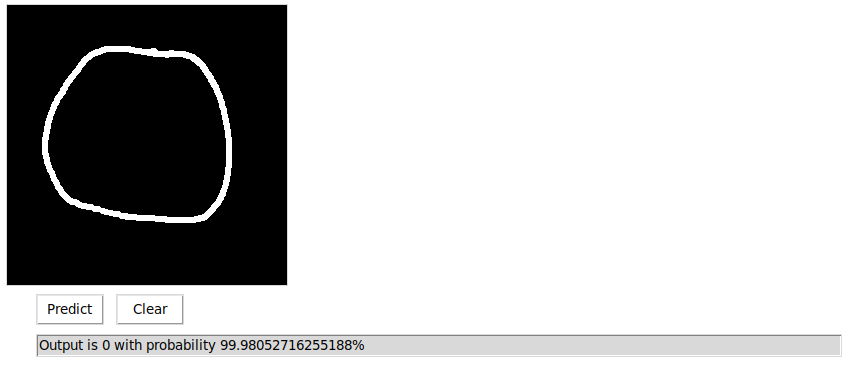
\includegraphics[scale = 0.5]{../figs/0.png}
    \end{figure}

    \begin{figure}[!ht]
        \centering
        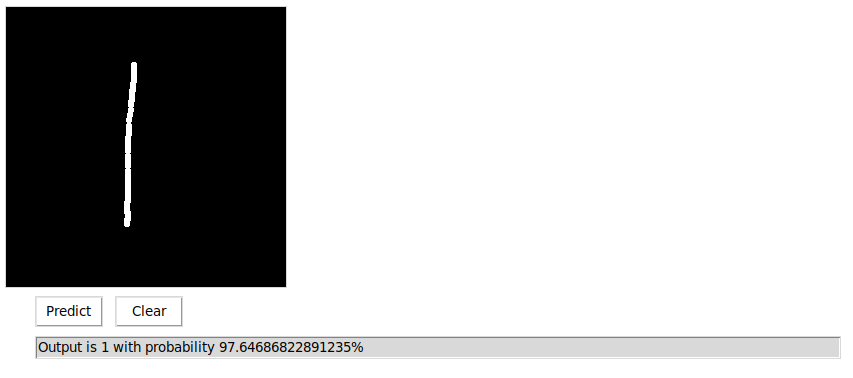
\includegraphics[scale = 0.5]{../figs/1.png}
    \end{figure}

    \begin{figure}[!ht]
        \centering
        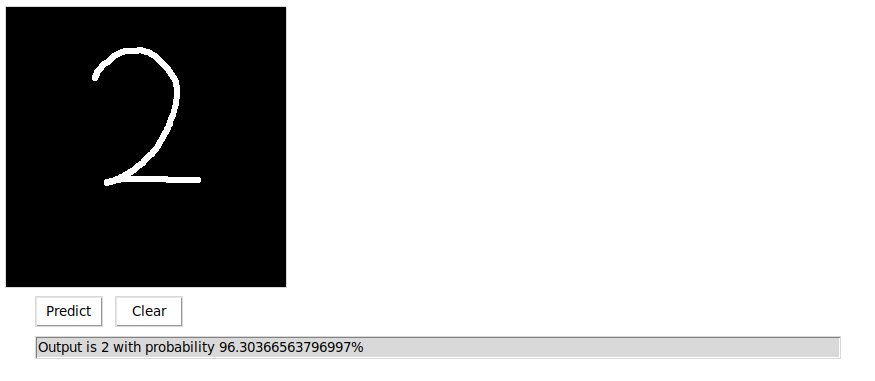
\includegraphics[scale = 0.5]{../figs/2.png}
    \end{figure}

    \begin{figure}[!ht]
        \centering
        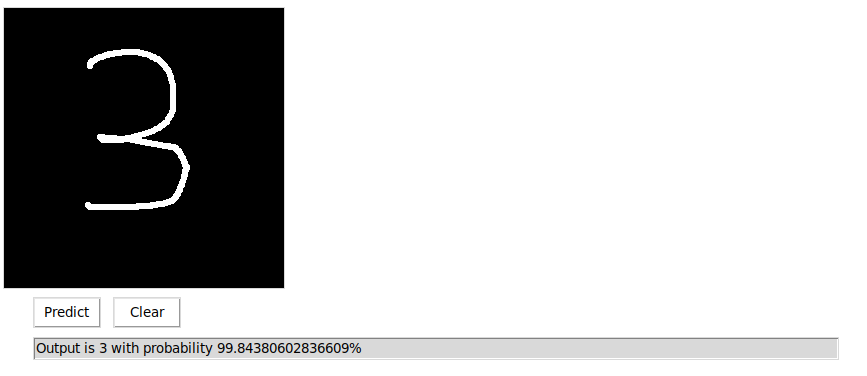
\includegraphics[scale = 0.5]{../figs/3.png}
    \end{figure}

    \begin{figure}[!ht]
        \centering
        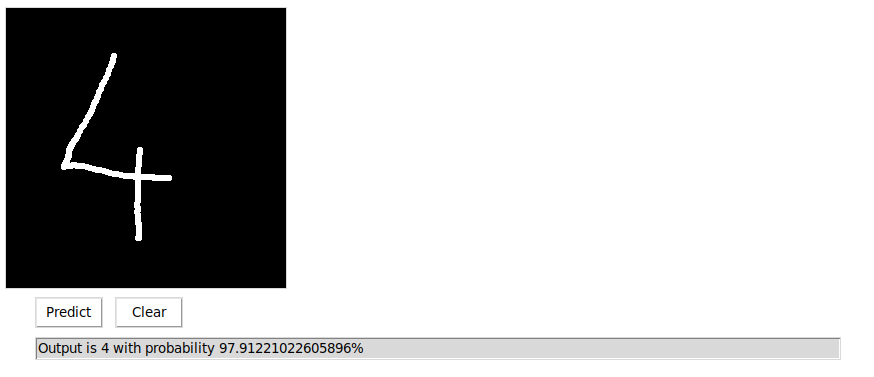
\includegraphics[scale = 0.5]{../figs/4.png}
    \end{figure}
    
    \begin{figure}[!ht]
        \centering
        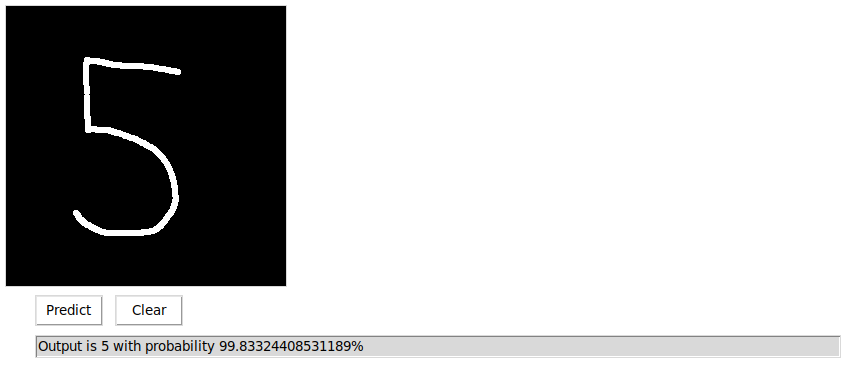
\includegraphics[scale = 0.5]{../figs/5.png}
    \end{figure}

    \begin{figure}[!ht]
        \centering
        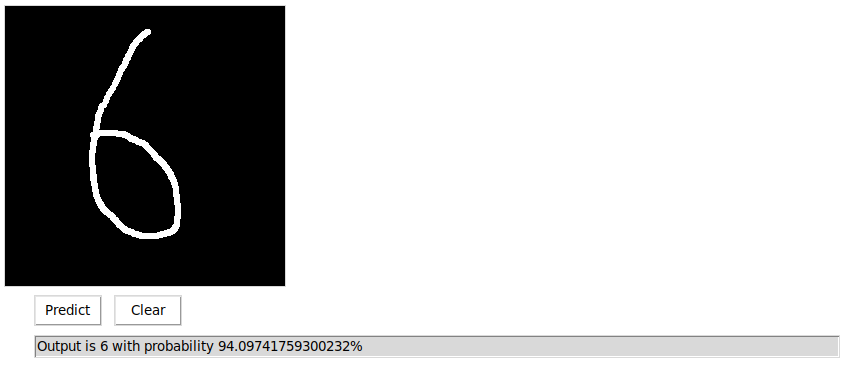
\includegraphics[scale = 0.5]{../figs/6.png}
    \end{figure}

    \begin{figure}[!ht]
        \centering
        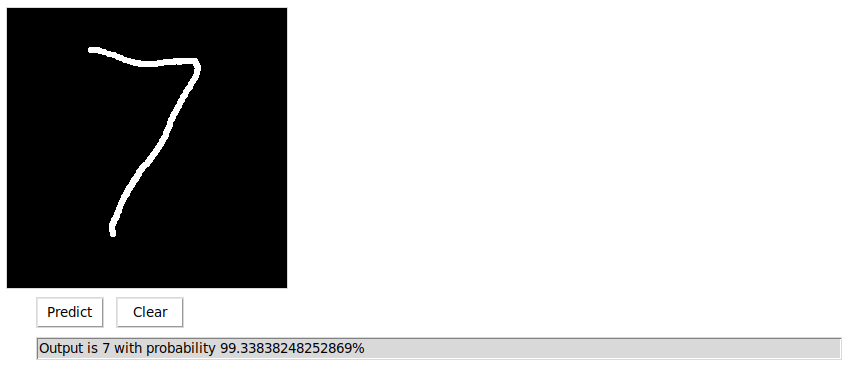
\includegraphics[scale = 0.5]{../figs/7.png}
    \end{figure}

    \begin{figure}[!ht]
        \centering
        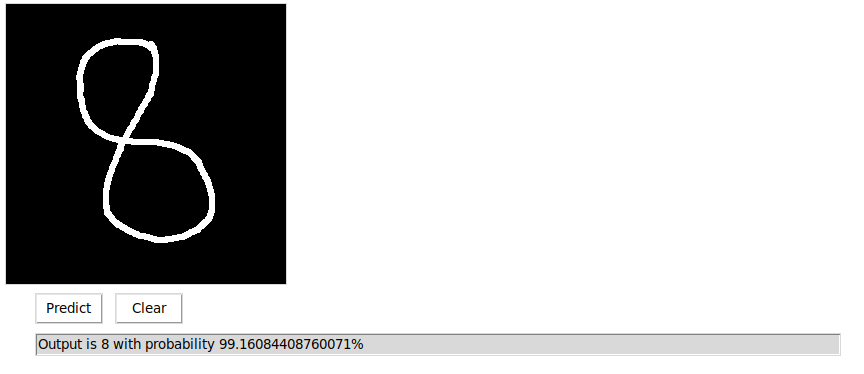
\includegraphics[scale = 0.5]{../figs/8.png}
    \end{figure}

    \begin{figure}[!ht]
        \centering
        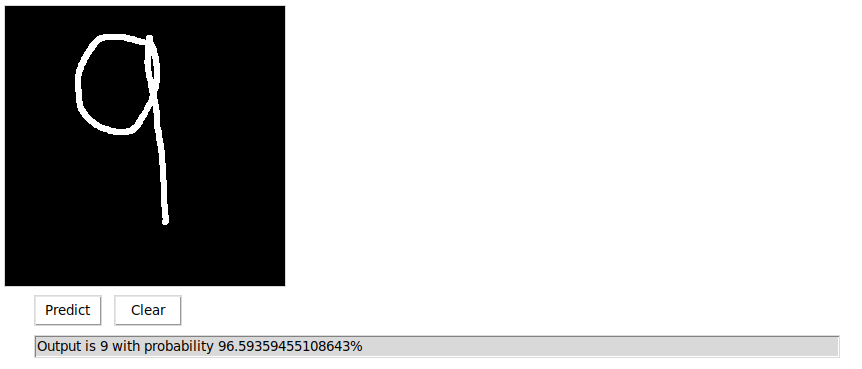
\includegraphics[scale = 0.5]{../figs/9.png}
    \end{figure}

\end{large}

\end{document}